
\section{Proposed Method}

In domain generalization for multi-label ocular disease recognition, model performance is mainly affected by three factors. First, multiple diseases may coexist in the same fundus image. If the model cannot effectively capture relevance among disease labels and between labels and disease-related features, false positives and false negatives may occur, degrading multi-label recognition performance. Second, distribution shifts commonly arise between the source domain and target domain. If the learned features contain substantial source-domain-specific noise, the transferability of disease-related features is weakened, resulting in poorer domain generalization performance. In addition, although privacy-preserving mechanisms can reduce privacy leakage risk, they may also affect model optimization through additional training constraints. The balance between privacy preservation and model performance must therefore be considered.

To address these issues, this study does not treat multi-disease co-occurrence and domain shift as separate problems. Instead, they are jointly modeled within a single domain generalization framework for multi-label ocular disease recognition. As shown in \hyperref[fig:method-framework]{Fig.~\ref*{fig:method-framework}}, the proposed interpretable single domain generalization framework consists of two main parts: Part 1, Dual-Branch Guided Domain-Invariant Feature Extraction (DFE), and Part 2, Adaptive Label-Feature Relevance Construction (ARC). Part 1 uses CAM guidance together with a dual-branch mask-based contrastive learning mechanism to extract more stable domain-invariant features from a single source domain, thereby reducing the influence of distribution shift between the source domain and unseen domains. CAM also visualizes model-attended regions and enhances interpretability. Based on the domain-invariant features produced by Part 1, Part 2 uses Transformer attention mechanisms to model label-label relevance and label-feature relevance, reducing false positives and false negatives in multi-label recognition. These two parts are coupled through feature filtering and attention consistency constraints: Part 1 provides more stable domain-invariant features for Part 2, while Part 2 further constrains the consistency of dual-branch attention features, jointly improving domain generalization performance. Finally, an Adaptive Gaussian Differential Privacy mechanism is integrated during training to reduce the impact of privacy preservation on model performance and to balance privacy preservation with model performance. Overall, the proposed method constructs a Privacy-Preserving Interpretable Single Domain Generalization framework for multi-label ocular disease recognition. The implementation details of each module are described in the following three subsections.

\begin{figure}[!htb]
\centering
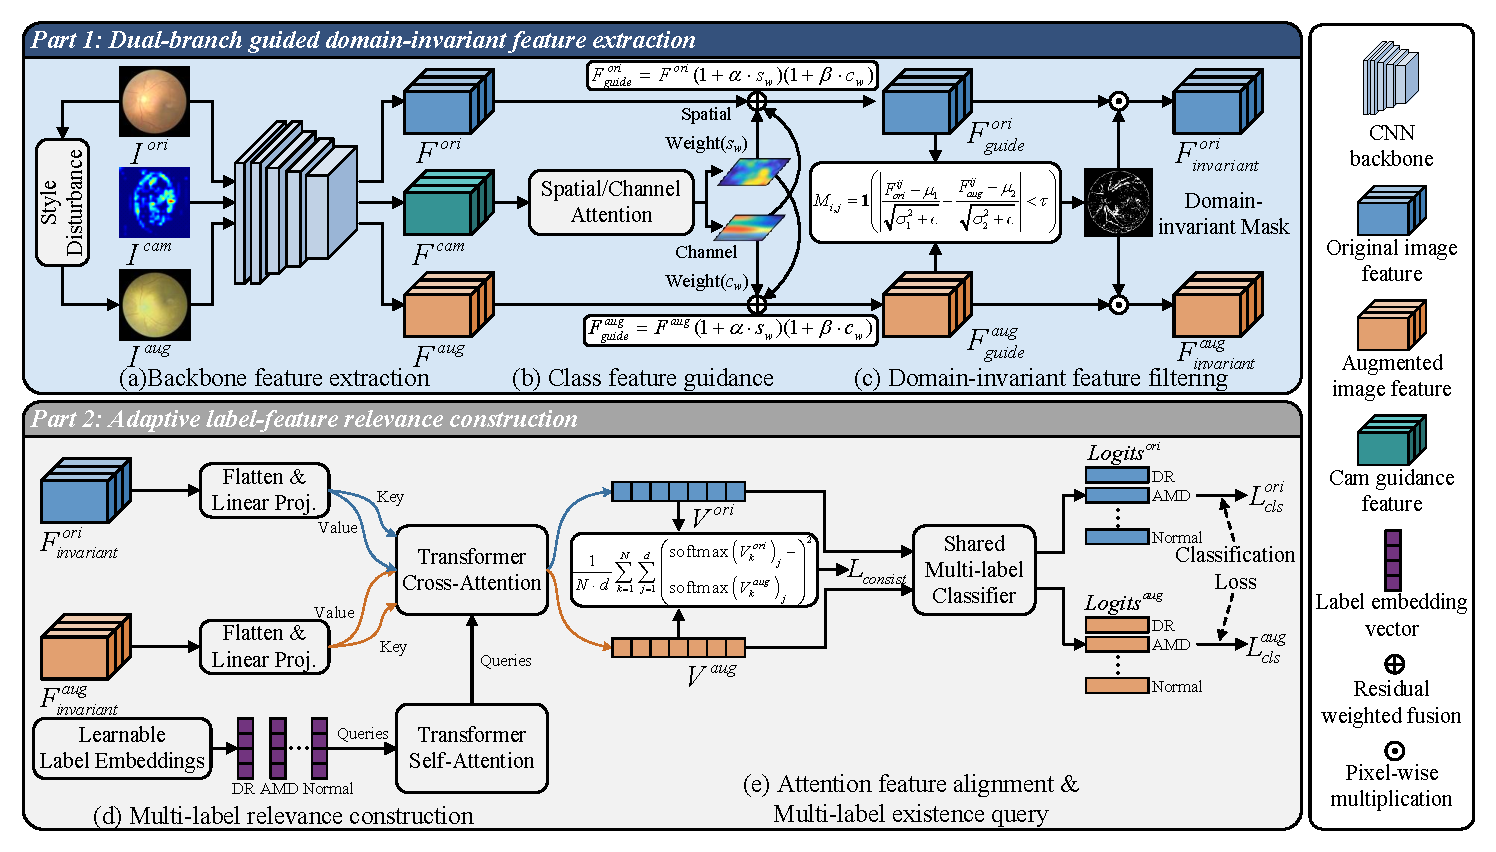
\includegraphics[width=0.96\textwidth]{./images/media/image2_padded.pdf}
\caption{Overview of the proposed interpretable single domain generalization framework. Part 1 is Dual-Branch Guided Domain-Invariant Feature Extraction (DFE), consisting of (a)--(c): (a) original source-domain images and augmented source-domain images are first fed into the backbone to extract dual-branch features; (b) CAM is used to generate model-attended region guidance, which enhances disease-related regions and suppresses background noise; and (c) a dual-branch mask-based contrastive learning mechanism retains highly similar components between the two feature branches to extract domain-invariant features. Part 2 is Adaptive Label-Feature Relevance Construction (ARC), consisting of (d)--(e): (d) Transformer self-attention is used to model label-label relevance, and cross-attention is then used to establish label-feature relevance; (e) attention consistency constraints improve the stability of attention features, thereby reducing false positives and false negatives in multi-label recognition. Part 1 and Part 2 work collaboratively, enabling the model to extract domain-invariant features while modeling label relevance more effectively, thus jointly improving domain generalization performance.}
\label{fig:method-framework}
\end{figure}

\letteredsubsection{A. Dual-Branch Guided Domain-Invariant Feature Extraction}

Considering that multi-institutional data in medical scenarios are often difficult to centralize or use synchronously, this study adopts a single domain generalization setting and learns domain-invariant features for unseen-domain data using only one source domain. Inspired by contrastive learning, original source-domain images are transformed into augmented source-domain images through augmentation techniques such as style disturbance to simulate possible distribution shifts in unseen domains. Specifically, \(I^{ori}\) denotes original source-domain images, and \(I^{aug}\) denotes augmented source-domain images generated by style disturbance, such as MixStyle or random adjustment of brightness, contrast, and saturation. This augmentation simulates differences in imaging devices, illumination environments, or patient populations in cross-domain scenarios while preserving the semantic content of the images, namely disease regions.

First, as shown in \hyperref[fig:method-framework]{Fig.~\ref*{fig:method-framework}.a}, both \(I^{ori}\) and \(I^{aug}\) are fed into the backbone network to extract features \(F^{ori}\) and \(F^{aug}\). Let \(F^{ori} \in \mathbb{R}^{C \times H \times W}\) and \(F^{aug} \in \mathbb{R}^{C \times H \times W}\), where \(C\), \(H\), and \(W\) denote the number of channels, height, and width of the final feature map of the backbone network, respectively. ResNet50 is selected as the backbone because it performs well in medical image classification and offers good feature extraction capability and computational efficiency. However, relying only on contrastive constraints between original and augmented source-domain images remains limited. The model may still learn domain-specific noise such as background textures, illumination variations, or image-edge artifacts, which can affect multi-label ocular disease recognition on unseen domains.

To this end, we introduce the class feature guidance module shown in \hyperref[fig:method-framework]{Fig.~\ref*{fig:method-framework}.b} to improve the disease relevance and interpretability of features. CAM is generated on the training set in advance using the baseline model, namely ResNet50 with BCE loss. CAM highlights the regions attended by the model for different diseases; for example, Diabetic Retinopathy (DR) mainly corresponds to vascular regions, whereas Age-related Macular Degeneration (AMD) mainly corresponds to the macular region. It is calculated as follows:

\[I^{cam} = \sum_{k = 1}^{C}w_{k} \cdot A_{k},
\]

Here, \(A_{k}\) is the activation map of the \(k\)-th channel in the last convolutional layer of the backbone network, and \(w_{k}\) is the weight obtained from the gradient of the classification weights after global average pooling. This formula follows a Grad-CAM variant and enables CAM to capture class-specific model-attended regions. The generated CAM \(I^{cam}\) is fed into the backbone network to obtain \(F^{cam} \in \mathbb{R}^{C \times H \times W}\). Spatial attention weights \(s_{w}\) and channel attention weights \(c_{w}\) are then computed from \(F^{cam}\) through spatial and channel attention modules, respectively. Both attention modules are convolutional sequential networks containing \(1 \times 1\) convolution, ReLU activation, and a Sigmoid function for adaptive weight generation. The spatial attention module additionally combines average and max pooling to capture local context, generating a pixel-level weight map that adaptively enhances the saliency of lesion regions, such as vessels or the macula, while suppressing background noise. The channel attention module uses adaptive average pooling to compress spatial dimensions and obtain global statistics, then learns channel dependencies to enhance disease-texture-sensitive channels and suppress noisy channels. The two weights are applied to \(F^{ori}\) and \(F^{aug}\) to obtain CAM-guided features \(F_{guide}^{ori}\) and \(F_{guide}^{aug}\). A residual connection is used in the weighting operation to avoid damaging original information through excessive guidance:

\[F_{guide}^{ori} = F^{ori}(1 + \alpha{\cdot s}_{w})(1 + {\beta \cdot c}_{w}),
\]\[F_{guide}^{aug} = F^{aug}(1 + \alpha{\cdot s}_{w})(1 + {\beta \cdot c}_{w}),\]

Here, \(\alpha\) and \(\beta\) are hyperparameters that control the enhancement strengths of \(s_{w}\) and \(c_{w}\), respectively. Residual weighting allows CAM guidance to highlight disease-related regions while retaining the original feature representation, reducing the model's reliance on domain-specific noise such as illumination and background textures. Extracting domain-invariant features from these guided representations helps improve feature disease relevance. Meanwhile, visualizing model-attended regions through CAM enhances model interpretability and helps clinicians understand the basis of prediction, for example by overlaying CAM to inspect whether the model focuses on lesion regions.

Next, we introduce the domain-invariant feature filtering module, as shown in \hyperref[fig:method-framework]{Fig.~\ref*{fig:method-framework}.c}. This study adopts a dual-branch mask-based contrastive learning mechanism to compute the similarity between guided features from original source-domain images and augmented source-domain images at the feature-distribution level. Highly similar components represent disease-related regions that remain stable under style disturbance and are therefore retained, whereas low-similarity components are more likely to contain domain-specific noise caused by illumination, device style, or style disturbance and are therefore suppressed. The mask matrix \(M \in \mathbb{R}^{C \times H \times W}\) is calculated from the normalized distance:

\[
M_{ij} =
\left\{
\begin{array}{ll}
1, & \text{if } \left| \dfrac{F_{guide}^{ori,ij} - \mu_{1}}{\sqrt{\sigma_{1}^{2} + \epsilon}} - \dfrac{F_{guide}^{aug,ij} - \mu_{2}}{\sqrt{\sigma_{2}^{2} + \epsilon}} \right| \leq \tau, \\
0, & \text{otherwise.}
\end{array}
\right.
\]

Here, \(\mu_{1},\sigma_{1}\) and \(\mu_{2},\sigma_{2}\) are the means and variances of the two guided features, respectively, \(\epsilon = 10^{-5}\) is a stability constant, and \(i,j\) denote feature map positions. Components satisfying the threshold \(\tau\) are assigned 1, while the remaining components are assigned 0. The mask matrix is then applied to \(F_{guide}^{ori}\) and \(F_{guide}^{aug}\) to extract domain-invariant features:

\[F_{invariant}^{ori} = F_{guide}^{ori} \odot M,F_{invariant}^{aug} = F_{guide}^{aug} \odot M,
\]

Here, \(\odot\) denotes pixel-wise element-wise multiplication, ensuring that only shared disease-related features, such as vascular or macular textures, are retained while illumination or device noise is removed. The resulting \(F_{invariant}^{ori}\) and \(F_{invariant}^{aug}\) are used as inputs for subsequent label-feature relevance construction, enabling multi-label relevance learning to be built on more stable domain-invariant features.

\letteredsubsection{B. Adaptive Label-Feature Relevance Construction}

After obtaining domain-invariant disease features, the model further handles the multi-label relevance problem caused by ocular disease co-occurrence. To this end, Transformer attention mechanisms are embedded to construct adaptive relevance at the label and feature levels for multi-label prediction. As shown in \hyperref[fig:method-framework]{Fig.~\ref*{fig:method-framework}.d} and \hyperref[fig:method-framework]{Fig.~\ref*{fig:method-framework}.e}, this module includes multi-label relevance construction and attention feature alignment.

First, the eight labels in the ODIR dataset, such as normal, DR, and AMD, are modeled as learnable vectors \(L = \lbrack L_{1},\ldots,L_{8}\rbrack \in \mathbb{R}^{8 \times d}\), where \(d = 512\) is the embedding dimension. These vectors are initialized from a random Gaussian distribution and optimized during training to characterize potential relevance among different disease labels. The label vectors are fed into the Transformer self-attention mechanism to model label relevance:

\[
V_{self} = \operatorname{softmax}\left(\frac{QK^{T}}{\sqrt{d_{k}}}\right)V,
\]

Here, \(Q = LW_{Q},K = LW_{K},V = LW_{V}\), where \(W_{Q},W_{K},W_{V}\) are learnable projection matrices and \(d_{k} = d/heads\) for multi-head attention with \(heads=8\). The self-attention output \(V_{self}\) captures label relevance, enabling different disease labels to interact dynamically according to co-occurrence patterns and visual evidence in the training data.

Next, a cross-attention mechanism is used to combine labels with domain-invariant features. Since Transformer requires sequential input, \(F_{invariant}^{ori}\) and \(F_{invariant}^{aug}\) output by Part 1 are first flattened and used as Key and Value, while the label vector \(V_{self}\) is used as Query for cross-attention calculation:

\[
V_{cross}^{ori} = \operatorname{softmax}\left(\frac{V_{self}W_{Q}(F_{invariant}^{ori}W_{K})^{T}}{\sqrt{d_{k}}}\right)(F_{invariant}^{ori}W_{V}),
\]

\(V_{cross}^{aug}\) is calculated in the same way. Through multi-layer cross-attention, labels are matched with corresponding disease features to form attention vectors \(V \in \mathbb{R}^{8 \times d}\), which highlight disease-related regions, for example by enhancing lesion regions through pixel-wise multiplication. In this process, each label vector is not matched with image features independently; instead, it queries image features based on the label relevance modeled by self-attention. The model can therefore focus on local lesion features corresponding to each disease while also using disease co-occurrence dependencies to support the prediction of other relevant labels, thereby reducing false positives and false negatives in multi-label recognition.

To ensure consistency between the outputs of the two branches, we introduce an attention consistency constraint and compute an attention consistency loss. Original source-domain images and augmented source-domain images share the same disease labels and differ only in style. Therefore, the corresponding label attention vectors should remain close. This loss encourages consistent attention features across the two branches, enabling the model to learn similar label-feature relevance from inputs with different styles. It is calculated using mean squared error (MSE):

\[
L_{consist} = \frac{1}{N \cdot d}\sum_{k = 1}^{N}\sum_{j = 1}^{d}
\left(
\operatorname{softmax}\left( V_{k}^{ori} \right)_{j}
-
\operatorname{softmax}\left( V_{k}^{aug} \right)_{j}
\right)^{2},
\]

Here, \(N = 8\) is the number of labels and \(d = 512\) is the embedding dimension. Softmax normalizes attention vectors into comparable distribution forms. The attention consistency loss improves model stability under domain shift by minimizing differences between normalized attention features of the two branches.

Finally, the attention vectors are fed into the multi-label classifier. LayerNorm and Dropout are first applied to the class query features for lightweight feature enhancement, normalization, and regularization. Class-wise linear transformations are then used to obtain logits for each class. After Sigmoid activation, the prediction probabilities \(p^{ori}\) are obtained for each class, and \(p^{aug}\) is obtained in the same way. The classification loss uses binary cross entropy (BCE):

\[L_{cls}^{ori} = - \frac{1}{8}\sum_{k = 1}^{8}{\lbrack y_{k}\log p_{k}^{ori} + (1 - y_{k})\log(1 - p_{k}^{ori})\rbrack},
\]

The total loss is \(L = L_{cls}^{ori} + L_{cls}^{aug} + \lambda L_{consist}\), where \(\lambda\) is a hyperparameter that balances the consistency term. Through this design, the DFE module provides disease-related domain-invariant features for the ARC module, and the ARC module further models label-label relevance and label-feature relevance. The two modules work together to improve multi-label recognition capability in cross-domain scenarios.

\letteredsubsection{C. Integration of Privacy Preservation}

Medical image data are highly sensitive, and gradients or model parameters generated during training may leak sample information. In particular, gradient inversion attacks may even recover original images, leading to privacy leakage risk. To balance privacy preservation and model performance in single domain generalization models, this study introduces an Adaptive Gaussian Differential Privacy (AdaGDP) mechanism. The overall privacy-preserving framework is shown in \hyperref[fig:privacy-framework]{Fig.~\ref*{fig:privacy-framework}}.

\begin{figure}[!htb]
\centering
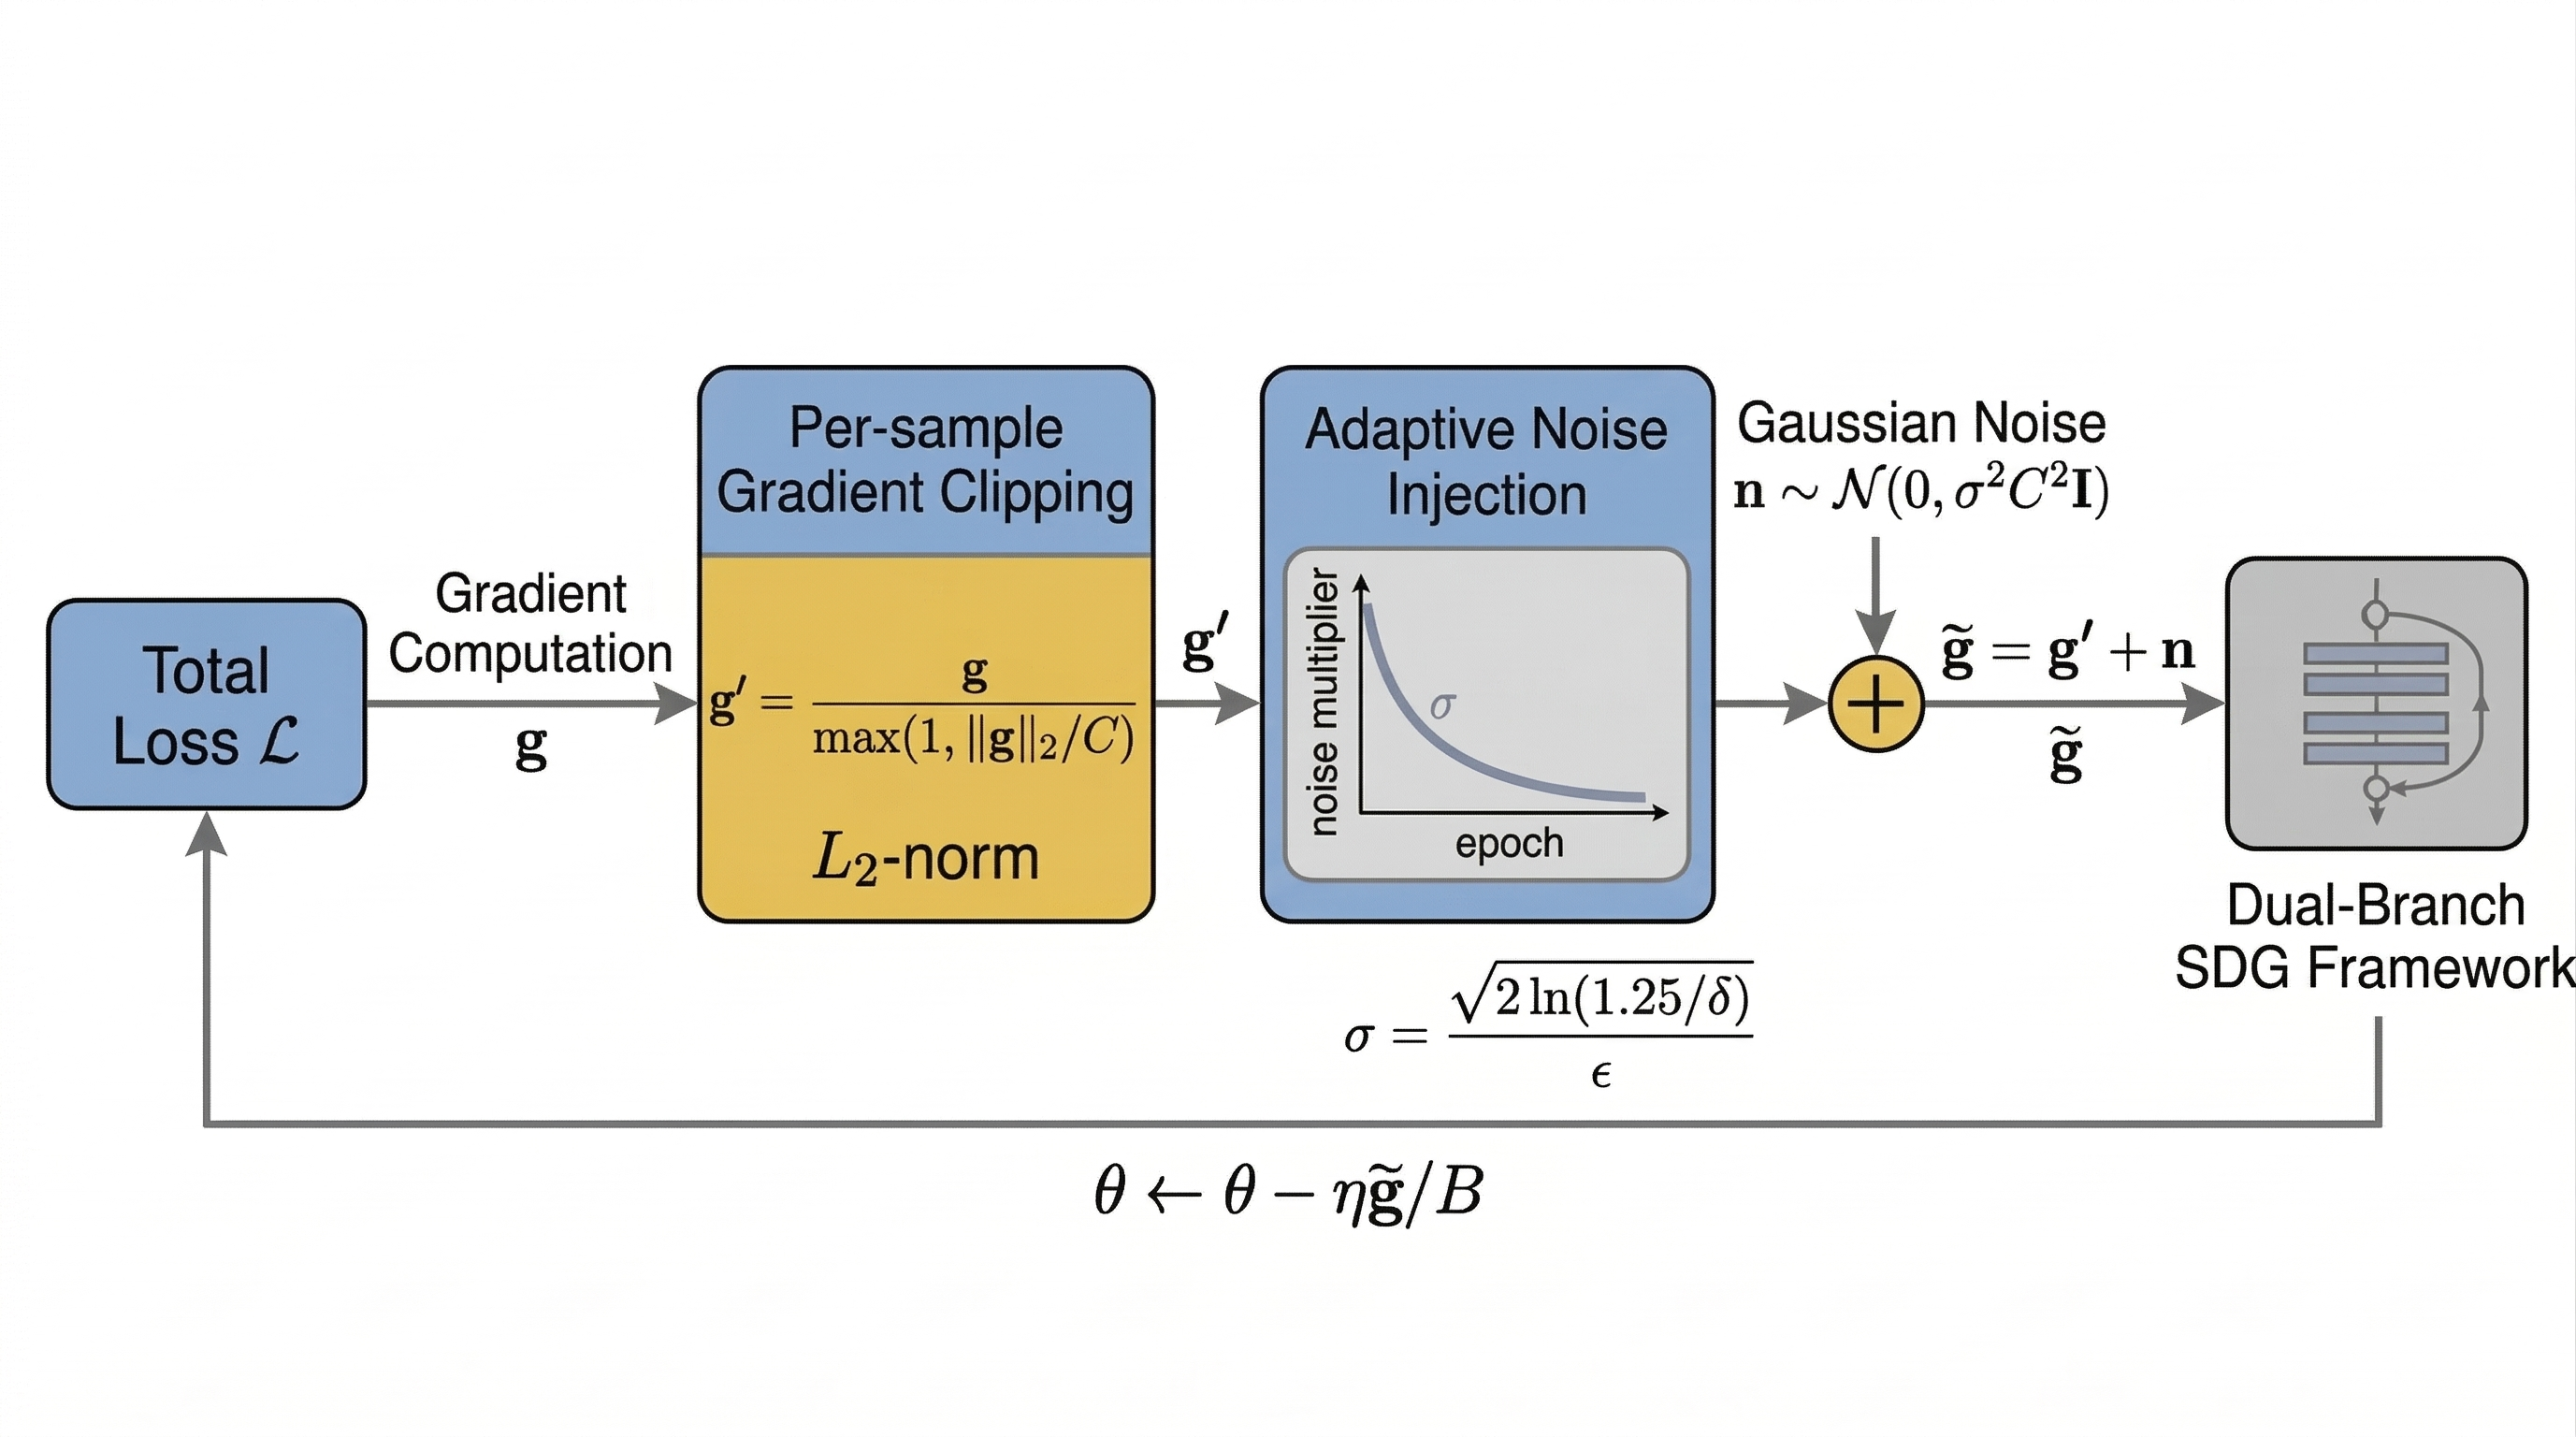
\includegraphics[width=0.82\textwidth]{./images/media/image3_v2.png}
\caption{Integration of Adaptive Gaussian Differential Privacy into the single domain generalization framework. During training, each update first clips per-sample gradients, then injects Gaussian noise and updates the parameters. Unlike fixed-noise differential privacy, this study adopts a noise multiplier that is adaptively adjusted and gradually decayed with the training stage, providing stronger privacy preservation early in training while reducing noise interference with model convergence in later stages, thereby achieving a privacy-performance trade-off.}
\label{fig:privacy-framework}
\end{figure}

Gaussian differential privacy (GDP) provides \((\epsilon, \delta)\)-differential privacy by adding independent and identically distributed Gaussian noise at each gradient update. For adjacent datasets \(D\) and \(D'\), which differ by only one sample, a randomized algorithm \(M\) satisfies \((\epsilon, \delta)\)-DP if, for any output set \(S\), it satisfies:

\[\Pr\lbrack M(D) \in S\rbrack \leq e^{\epsilon}\Pr\lbrack M(D') \in S\rbrack + \delta,
\]

where \(\epsilon\) measures the degree of privacy preservation, and \(\delta\) is the relaxation parameter, usually set to \(10^{-5}\). Under the DP-SGD framework, the per-sample gradient \(g\) is first clipped by its L2 norm at each iteration:

\[g' = g/max(1, \parallel g \parallel_{2}/C),
\]

Gaussian noise \(n \sim \mathcal{N}(0,\sigma^{2}C^{2}I)\) is then added, where \(\sigma\) is the noise multiplier controlling noise intensity. It is usually related to the privacy budget \(\epsilon\) and relaxation parameter \(\delta\), and can be written as:

\[\sigma = \sqrt{2\ln(1.25/\delta)}/\epsilon.
\]

The noisy gradient is \(\widetilde{g} = g' + n\), and the parameters are updated as \(\theta \leftarrow \theta - \eta\widetilde{g}/B\), where \(B\) is the batch size. This process obscures gradients through noise injection and prevents inversion attacks from recovering original images or labels. Detailed theoretical guarantees for privacy-preserving mechanisms are provided by Dwork C et al.\hyperref[_Ref214903493]{{[}45{]}}.

However, conventional GDP uses a fixed \(\sigma\) throughout training, so substantial noise is still injected in later training stages, which can affect model convergence and final performance. Therefore, we adopt an Adaptive Gaussian Differential Privacy optimizer. A larger noise multiplier is used early in training to provide stronger protection, and the noise intensity is then gradually reduced according to a predefined noise decay rate to limit the impact of noise on model convergence in later stages. During training, this study accumulates the privacy budget according to the noise multiplier, noise decay rate, and sampling process of each epoch, and records \(\epsilon\) consumption and model performance at different training epochs to analyze performance evolution as the privacy budget increases. The final experiments show that, under a moderate privacy budget, the proposed method can alleviate the performance degradation caused by noise injection and achieve a good balance between privacy preservation and model performance.
